\chapter{Introduction}

In natural language processing, it is frequently necessary to judge the
correctness of sentences generated by some algorithm. For example, a
speech-to-text translator that only recognizes individual words might produce
the following two candidate sentences for the same input audio sample:
\begin{align*}
 \text{He ate soup.} &&
 \text{He aid soup.}
\end{align*}

Both sentences sound the same, but the second candidate sentence should be
discarded because it is syntactically wrong. As another example, a translation
algorithm that translates from another language to English might generate the
following two candidate sentences for some input text:
\begin{align*}
 \text{This is a small red ball.} &&
 \text{This is a red small ball.}
\end{align*}

Both sentences are syntactically correct, but the first sentence should be
preferred because it conforms to the customary rules for adjective ordering in
the English language. Finally, consider a spelling correction process that is
applied to the following sentence:
\begin{align*}
 \text{The design \textbf{an} construction of the system will take more than a year. \cite{kukich1992}}
\end{align*}

Possible replacements for the syntactically wrong word ``an'' include ``a'' and
``and''. In all these situations, a \emph{language model} can be employed to
choose the best result from a set of candidates.
\cite{stolcke2002,youngetal2005} A language model assigns a probability $p_\omega(v)$
to each sentence $v\in V^*$ (with words from the set $V$), such that
correct sentences receive a higher probability than incorrect sentences, e.~g.,
\[
 1 > p_\omega\mbig\kla{\text{He ate soup.}} > p_\omega\mbig\kla{\text{He aid soup.}} > p_\omega\mbig\kla{\text{He He He soup.}} > 0.
\]

The probability distribution $p_\omega$ is determined by a \emph{model
parameter} $\omega\in\Omega$. The language model defines $\Omega$ and describes
how to obtain $p_\omega$ for any model parameter $\omega$. The model parameter
is chosen by a suitable \emph{training algorithm} using a training corpus $c$
containing known good sentences, such that $\omega$ maximizes the likelihood of
this corpus, i.~e.,
\[
 \prod_{v\in c} p_\omega(v).
\]

Many training algorithms for language models are instances of the
\emph{expectation-ma\-xi\-mi\-za\-tion (EM) algorithm} \cite{demlairub77}. Chapter 2
will introduce a general framework for EM algorithms that first appeared in
\cite{bucstuvog15}.

\section{N-gram models}

\begin{figure}[b]
 \centering
 \begin{tikzpicture}
  \begin{scope}[every node/.style={rectangle,draw,minimum height=1.8em,minimum width=4em}]
   \node [minimum width=2em] (v0) at (-3,1) {\strut \#};
   \node (v11) at (0,0) {\strut He};
   \node (v12) at (0,2) {\strut She};
   \node (v21) at (4,0) {\strut ate};
   \node (v22) at (4,2) {\strut drank};
   \node (v31) at (7,0) {\strut soup}; %TODO: this word is misaligned because of its underlength
   \node (v32) at (7,2) {\strut tea};
   \node [minimum width=2em] (v4) at (10,1) {\strut \#};
  \end{scope}
  \begin{scope}[every node/.style={circle,inner sep=0.2ex},thick,>=stealth]
   \draw[->] (v0.east) -- node[auto,swap] {$0.5$} (v11.west);
   \draw[->] (v0.east) -- node[auto] {$0.5$} (v12.west);
   \draw[->] (v11.east) -- node[auto,swap] {$0.5$} (v21.west);
   \draw[->] ($(v12.east)!0.5!(v12.south east)$) -- node[auto,pos=0.35,swap] {$0.5$} ($(v21.north west)!0.5!(v21.west)$);
   \draw[->] ($(v11.east)!0.5!(v11.north east)$) -- ($(v22.south west)!0.5!(v22.west)$);
   \draw[->] (v12.east) -- node[auto] {$0.5$} (v22.west);
   \draw[->] (v21.east) -- node[auto,swap] {~$1$~} (v31.west);
   \draw[->] ($(v22.east)!0.5!(v22.south east)$) -- node[auto,swap] {$0.3$} ($(v31.north west)!0.5!(v31.west)$);
   \draw[->] (v22.east) -- node[auto] {$0.7$} (v32.west);
   \draw[->] (v31.east) -- node[auto,swap] {~$1$~} ($(v4.south west)!0.8!(v4.west)$);
   \draw[->] (v32.east) -- node[auto] {~$1$~} ($(v4.north west)!0.8!(v4.west)$);
  \end{scope}
 \end{tikzpicture}
 \caption{Graphic representation of an example instance of the bigram model.
 The nodes are words from the vocabulary $V\cup\{\#\}$. The start/end marker
 $\#$ is shown twice for readability's sake. Arrows $v\to v'$ represent a
 nonzero bigram probability $b(v'|v)$.\label{fig:01-bigram}}
\end{figure}

One of the simplest language models is the \emph{bigram model}.
\cite{vogler2015} It interprets the generation of a sentence as a stochastic
process, wherein each word is chosen with a probability conditional on the word
that appeared before it: (see~Figure~\ref{fig:01-bigram})
\[
 p(\text{He ate soup.}) = b(\text{He}|\#) \cdot b(\text{ate}|\text{He}) \cdot b(\text{soup}|\text{ate}) \cdot b(\#|\text{soup}).
\]
The model parameter is $b$, a conditional probability distribution of
$V\cup\brc{\#}$ given $V\cup\brc{\#}$ and $\#$ is a placeholder word
that stands in for the start and end of the sentence.

The model parameter $b$ can be chosen by a very simple training algorithm
\cite[pp.~123]{jm09}: All bigrams, i.~e., pairs of words occurring one after the
other, are counted across the corpus. This includes bigrams containing the
sentence delimiter word $\#$. Then, the counts are normalized into a
conditional probability distribution by setting
\[
 b(w|w') := \frac{\operatorname{count}(w'w)}{\sum_{w''\in V\cup\brc{\#}} \operatorname{count}(w'w'')}
 \quad\forall w,w'\in V\cup\brc{\#}.
\]

The bigram model can be generalized to the \emph{N-gram model}, wherein the
next word is chosen with a probability conditional on the $n-1$ words before
it. Training then counts $n$-grams, i.~e., sequences of $n$ words, hence the
name \emph{N-gram model}. The bigram model is recovered for $n=2$.

Besides the already mentioned applications where language models augment
translators and autocorrect systems, N-gram models are useful in
\emph{augmentive communication}: Virtual keyboards on smartphones and tablets
predict the next word by looking at the previous $n$ words, thus improving
typing speed and accuracy.  \cite{hasan2004n} A similar assistive word
prediction system is part of speech synthesis programs used by disabled persons
such as the physicist Stephen Hawking. \cite{newelletal1998}

\section{Hidden Markov model}

\begin{figure}[b!]
 \centering
 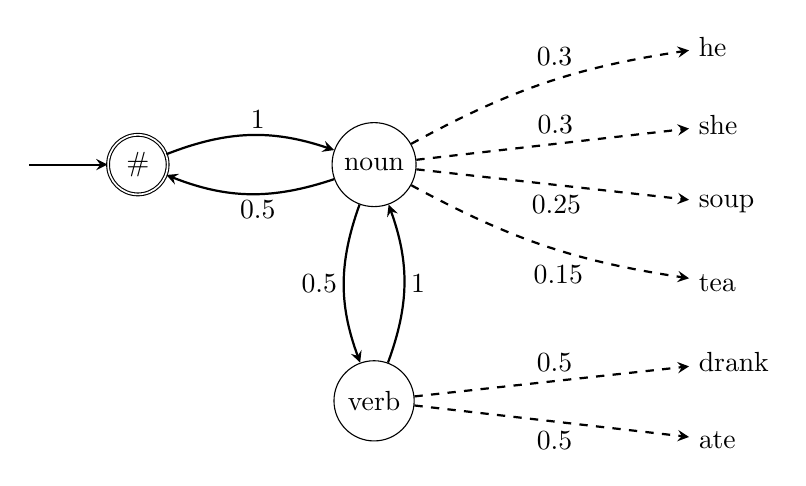
\begin{tikzpicture}[baseline=(current bounding box.north)]
  \begin{scope}[every node/.style={circle,draw}]
   \node[double] (q0) at (-3,3) {\#};
   \node (q1) at (0,3) {noun};
   \node (q2) at (0,0) {verb};
  \end{scope}
  \begin{scope}[every node/.style={anchor=west}]
   \node (v11) at (4,4.5) {he};
   \node (v12) at (4,3.5) {she};
   \node (v13) at (4,2.5) {soup};
   \node (v14) at (4,1.5) {tea};
   \node (v21) at (4,0.5) {drank};
   \node (v22) at (4,-0.5) {ate};
  \end{scope}
  \begin{scope}[every node/.style={rectangle,inner sep=0.5ex},thick,>=stealth]
   \draw[<-] (q0.west) -- +(-1,0);
   \draw[->] (q0) edge[bend left=20] node[auto,pos=0.55] {$1$} (q1);
   \draw[->] (q1) edge[bend right=20] node[auto,swap] {$0.5$} (q2);
   \draw[->] (q1) edge[bend left=20] node[auto,pos=0.45] {$0.5$} (q0);
   \draw[->] (q2) edge[bend right=20] node[auto,swap] {$1$} (q1);
   \draw[dashed,->] (q1) edge[bend left=10] node[auto,pos=0.63] {$0.3$} (v11);
   \draw[dashed,->] (q1) edge node[auto,pos=0.6] {$0.3$} (v12);
   \draw[dashed,->] (q1) edge node[auto,pos=0.63,swap] {$0.25$} (v13);
   \draw[dashed,->] (q1) edge[bend right=10] node[auto,pos=0.67,swap] {$0.15$} (v14);
   \draw[dashed,->] (q2) edge node[auto,pos=0.6] {$0.5$} (v21);
   \draw[dashed,->] (q2) edge node[auto,pos=0.6,swap] {$0.5$} (v22);
  \end{scope}
 \end{tikzpicture}
 \caption{Graphic representation of an example instance of the Hidden Markov
 model, with the hidden states ``noun'' and ``verb''; adapted from
 \cite{nel13}. Arrows $q\to q'$ represent nonzero transition probabilities
 $t(q'|q)$. Dashed arrows $q\dashrightarrow v$ represent nonzero emission
 probabilities $e(v|q)$.\label{fig:01-hmm}}
\end{figure}

A further generalization of N-gram models leads to the \emph{Hidden Markov
model}. In this model, the emission probability of a word depends not on the
previous words, but on the progression of a state machine that is not visible
from the outside. Every time a word needs to be emitted, the state machine
progresses to a new state according to a transition probability distribution
$t$ dependent on the previous state, and the next word is predicted by an
emission probability distribution $e$ dependent on the new state. The symbol
$\#$ is used as the initial and final state of the state machine.
\pagebreak % for figure to appear here

For example, if the state sequence that generated the sentence ``He ate soup''
was ``\#-noun-verb-noun-\#'', then the probability of that sentence would be
\begin{align*}
 p(v|q)
  =&\; t(\text{noun}|\#) \cdot e(\text{he}|\text{noun}) \cdot t(\text{verb}|\text{noun}) \cdot e(\text{ate}|\text{verb}) \\
  &\cdot t(\text{noun}|\text{verb}) \cdot e(\text{soup}|\text{noun}) \cdot t(\#|\text{noun}).
\end{align*}

Since the state sequence is typically not known, a sum over all possible state
sequences must be computed to obtain $p(v)$ for a sentence $v\in V^*$.

N-gram models can be interpreted a special case of the Hidden Markov model, by
encoding the current N-gram in the state ($Q = V^n$) and defining the
transmission and emission probability in terms of the N-gram probability. For
example, for bigrams,
\begin{align*}
 t(v_1v_2|v_1'v_2') &:= \begin{cases}
  b(v_2|v_1) & \text{if } v_1 = v_2', \\
  0 &\text{otherwise},
 \end{cases} &
 e(v|v_1v_2) &:= \begin{cases}
  1 & \text{if } v = v_2, \\
  0 &\text{otherwise}.
 \end{cases}
\end{align*}

Training for the Hidden Markov model is not as straightforward as for the
bigram model, since the training corpus typically only contains the observed
sentences, not the state sequences that produced them. The standard training
algorithm for Hidden Markov models is the \emph{Baum-Welch algorithm}.
\cite{baupetsouwei70,baum1972}

Chapter 3 will define Hidden Markov models more formally, and discuss
algorithms that act on them. Chapter 4 will specifically focus on the
Baum-Welch algorithm, and show that it is an instance of the general EM
algorithms laid out in chapter 2.
